\documentclass[a4paper,8pt,twocolumn]{article}
\usepackage[UTF8]{ctex}
\usepackage{graphicx}
\usepackage{fancyhdr}
\usepackage{amsmath}
\usepackage[
  left=2cm, 
  right=2cm,
  top=1.5cm,
  bottom=2.5cm
]{geometry}

\begin{document}

\title{
  \textbf{\huge 真实透镜仿真}}
\author{
  黄雨~24352027\\
\small 中山大学物理学院~广东~广州
}

\maketitle

\section{实验题目}
 1. 在给定的入射波长分别为 \textbf{532nm}、\textbf{632.8nm}、\textbf{587.6nm} 三个波长的工程中，  
 根据透镜的材料，正确计算对应波长的折射率；并分别找到其对应的焦点位置和焦距，调节【球面透镜】的 $L_1$ 和 $L_2$ 两个参数，使在焦点处成像。

 2. 另外有 \textbf{波长为587.6nm的二条光路}，光源输出为一个边长为 20mm 的五角星，同样计算该波长的折射率，调节对应【球面透镜】的 $L_1$ 和 $L_2$ 两个参数，使其中一条光路最终成像放大一倍，另一条光路最终成像缩小一倍，即：
 \begin{enumerate}
  \item 合理设置参数，得到缩小一倍的像，即五角星的边长为 10mm，且边缘清晰。
  \item 合理设置参数，得到放大一倍的像，即五角星的边长为 40mm，且边缘清晰。
 \end{enumerate}

\section{实验原理}
 由题目条件，空气折射率$n_0 = 1$，透镜折射率为$n_L$，系统矩阵为$S$，透镜厚度$T$，横向放大率$m$，如下：
 \begin{eqnarray*}
    S &=& S_3*S_2*S_1 \\
      &=&
    \left[
    \begin{array}{cc}
     1 & 0 \\
     \frac{n_L-n_0}{n_0R_2} & \frac{n_L}{n_0} \\
    \end{array}
    \right]
    \left[
    \begin{array}{cc}
     1 & T \\
     0 & 1 \\
    \end{array}
    \right]
    \left[
    \begin{array}{cc}
     1 & 0 \\
     \frac{n_0-n_L}{n_LR_1} & \frac{n_0}{n_L} \\
    \end{array}
    \right] \\
 \end{eqnarray*}

 \subsection{给定条件求焦距}
 当顶物距趋于无穷时，顶像距即为焦距，顶物距与顶像距转换关系如下：\\
  $$
  s' = - \frac{S_{12}*s - S_{12}}{S_{21}*s - S_{22}}
  $$

 \subsection{由横向放大率求顶物距和顶像距}
 \noindent
  通过系统矩阵，给定横向放大率，可求得顶像距为：\\
  $$
  s' = - \frac{m-S_{11}}{S_{21}}
  $$
  由顶像距和横向放大率，顶物距为：\\
  $$
  s = \frac{s'}{m}
  $$

  \subsection{仿真搭建}
  \noindent
  仿真搭建如图所示，详细数据参考工程文件
  \begin{figure}[h] 
    \centering
    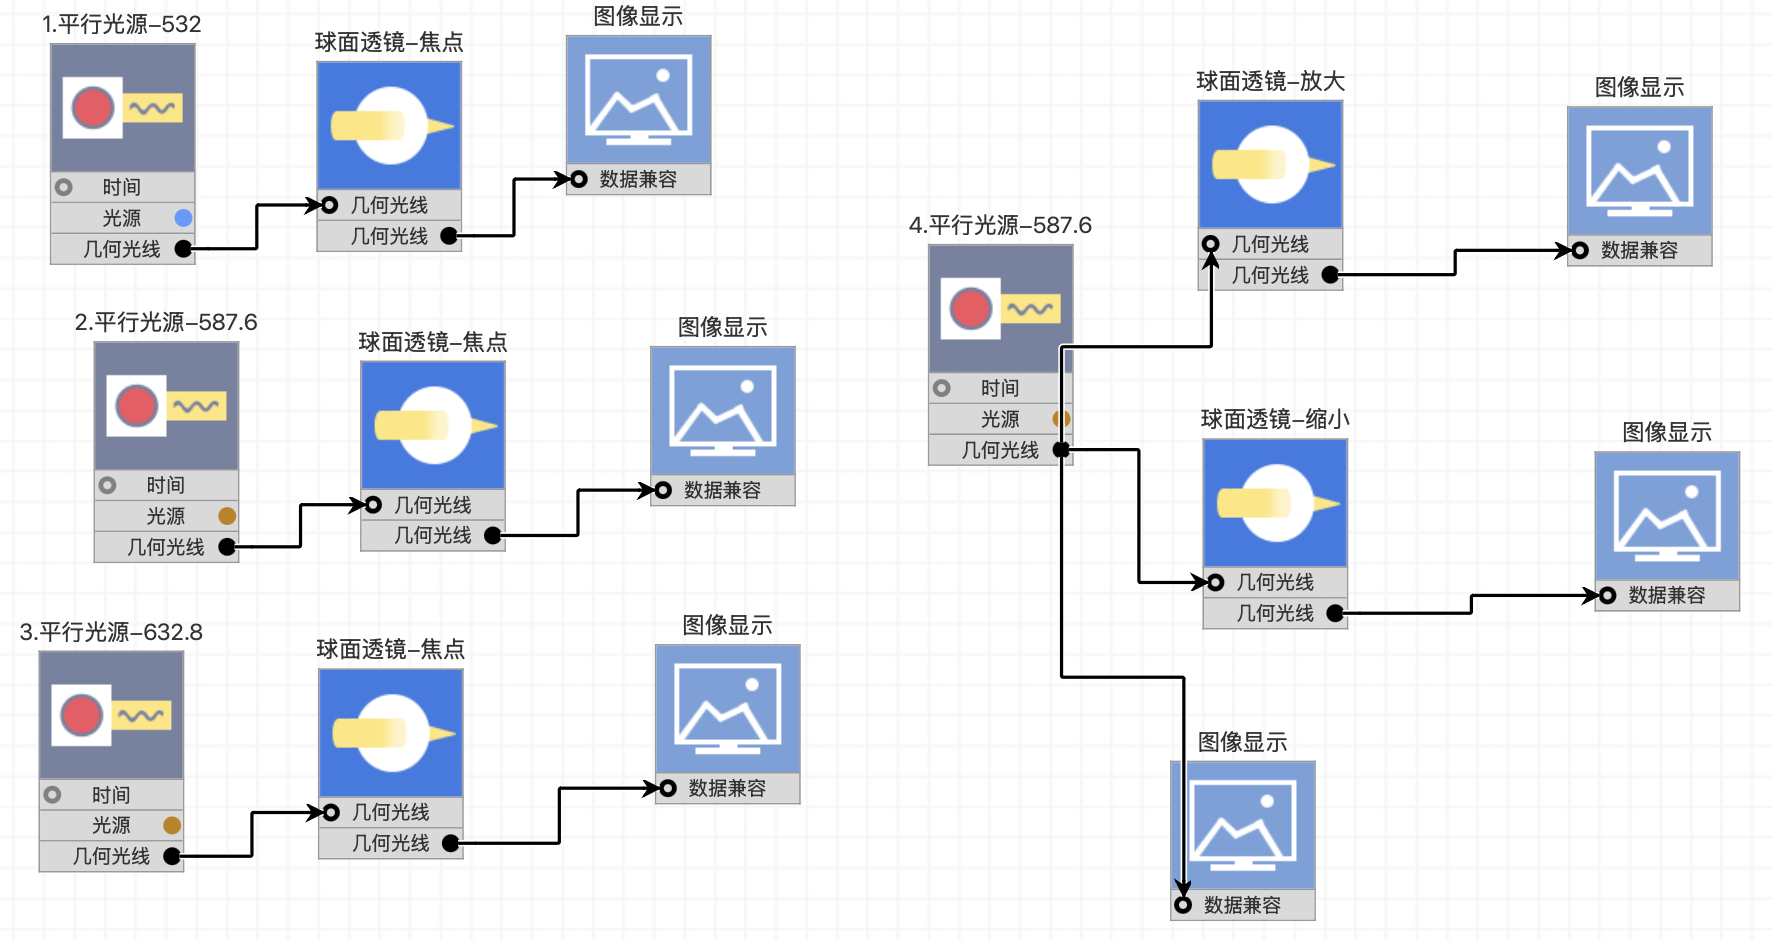
\includegraphics[width=0.5\textwidth]{Figure_2.1.png} 
    \caption{仿真搭建示意图}
    \label{Figure_2.1} 
  \end{figure}

\section{实验操作}
 \subsection{给定条件求焦距}
 令顶物距为$1000000~mm$，使用折射率计算器计算，得到对于不同波长的光线，相关数据如下：\\
 \begin{table}[h]
  \centering
   \begin{tabular}{|c|c|c|c|c|}
    \hline
    $\lambda/nm$ & $n_L$ & $R_1/mm$ & $R_2/mm$ & $L_2/mm$ \\ 
    \hline
    $532$ & $1.5194$ & $-131.5$ & $-49.1$ & $149.8993$ \\
    \hline
    $587.6$ & $1.5167$ & $-131.6$ & $-49.1$ & $150.6118$ \\
    \hline
    $632.8$ & $1.5151$ & $-131.6$ & $-49.1$ & $151.1134$ \\
    \hline
  \end{tabular}
  \caption{实验一数据}
  \label{Date_1}
 \end{table}\\

 输入上述数据后，得到仿真图像为：\\
 \begin{figure}[h] 
    \centering
    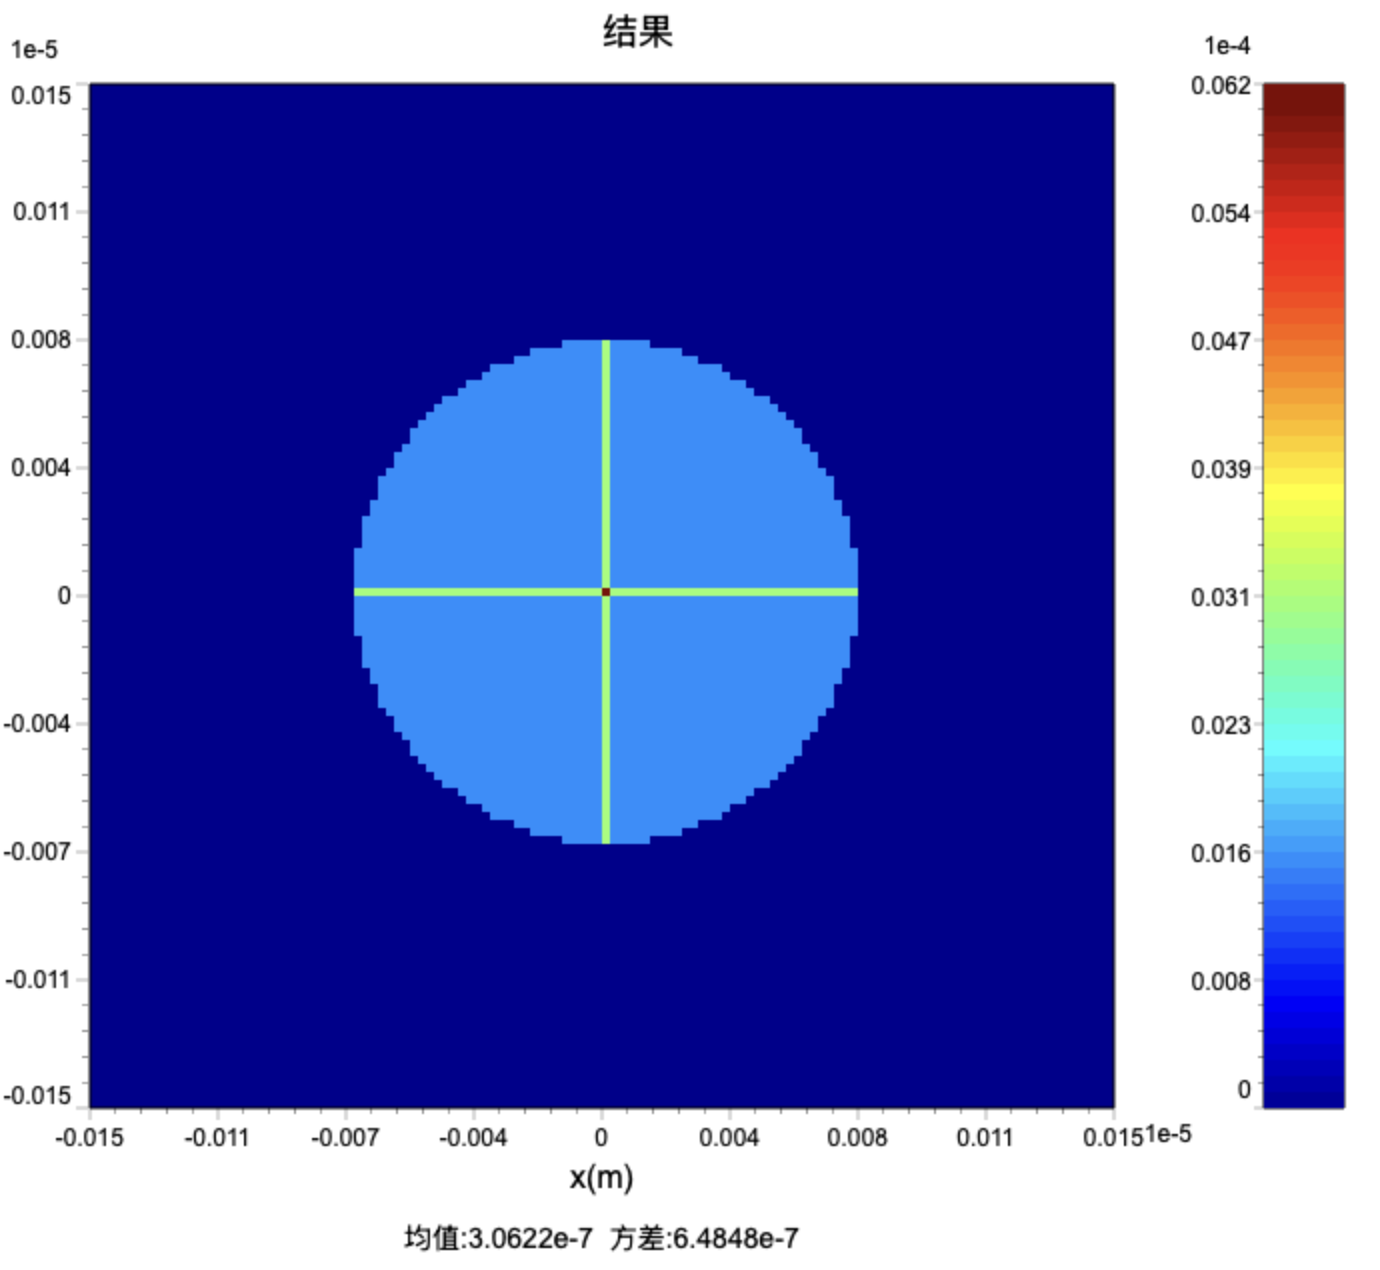
\includegraphics[width=0.3\textwidth]{Figure_3.1.png} 
    \caption{$532~nm$图像}
    \label{Figure_3.1} 
 \end{figure}
 \begin{figure}[h] 
    \centering
    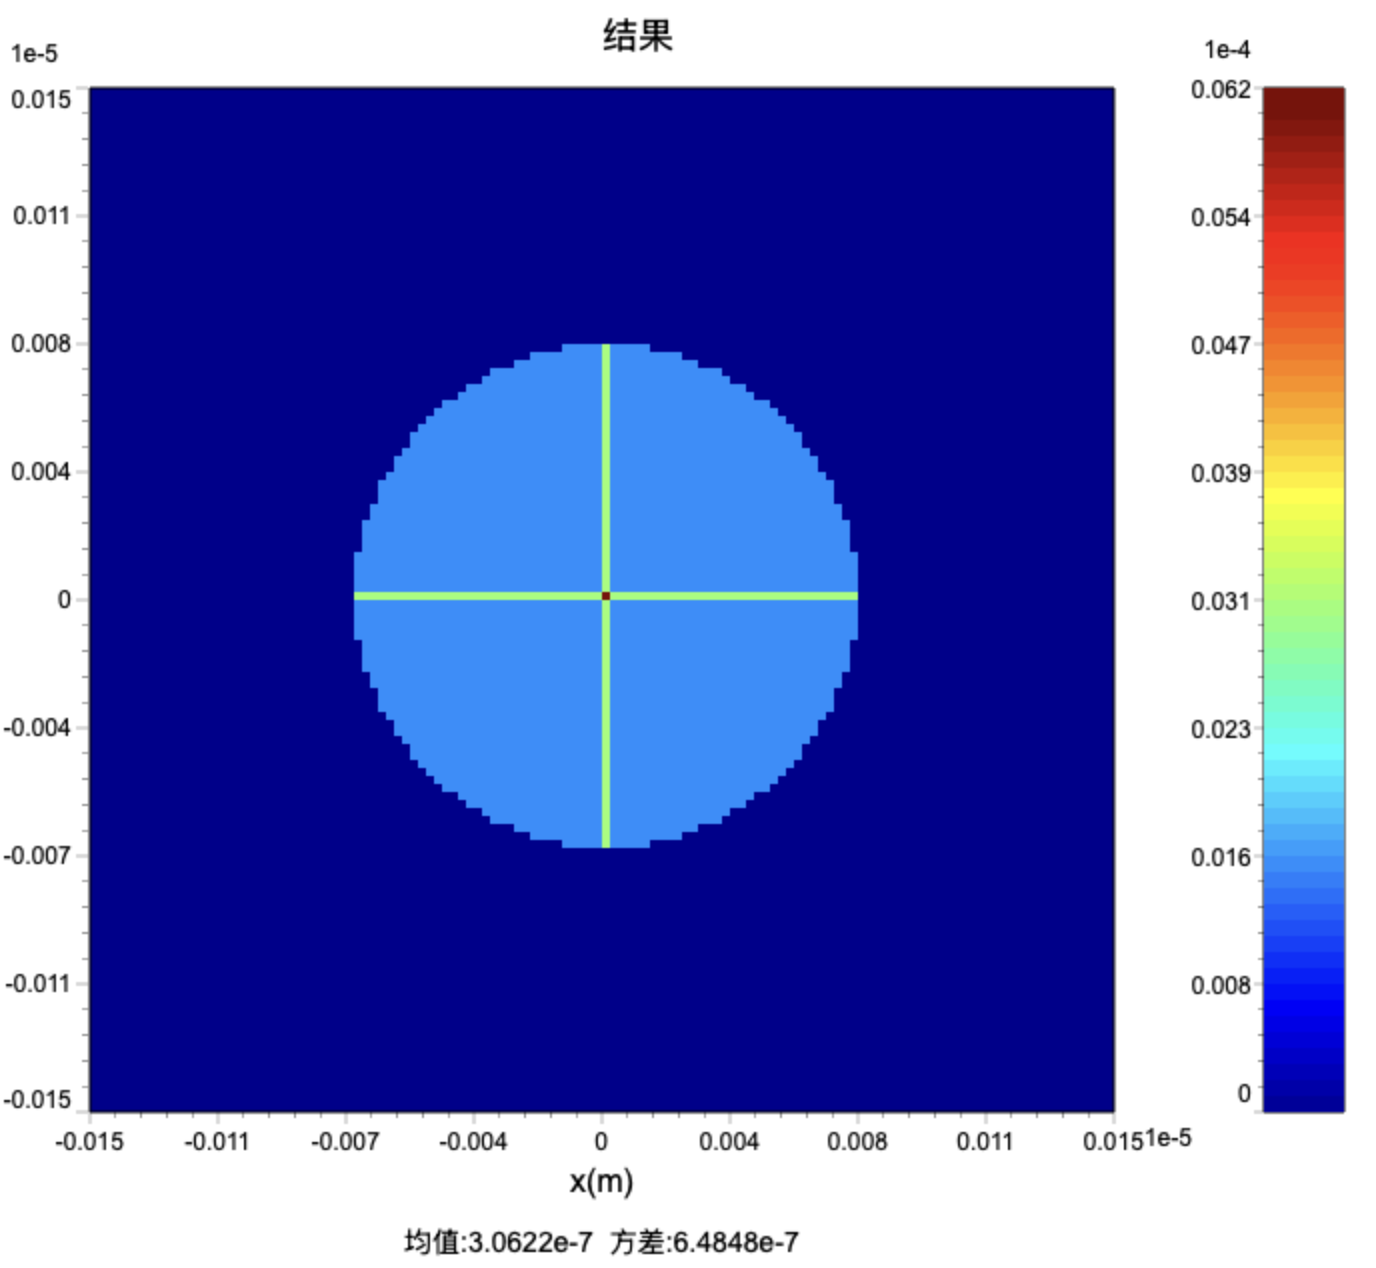
\includegraphics[width=0.3\textwidth]{Figure_3.2.png} 
    \caption{$587.6~nm$图像}
    \label{Figure_3.2} 
 \end{figure}
 \begin{figure}[h] 
    \centering
    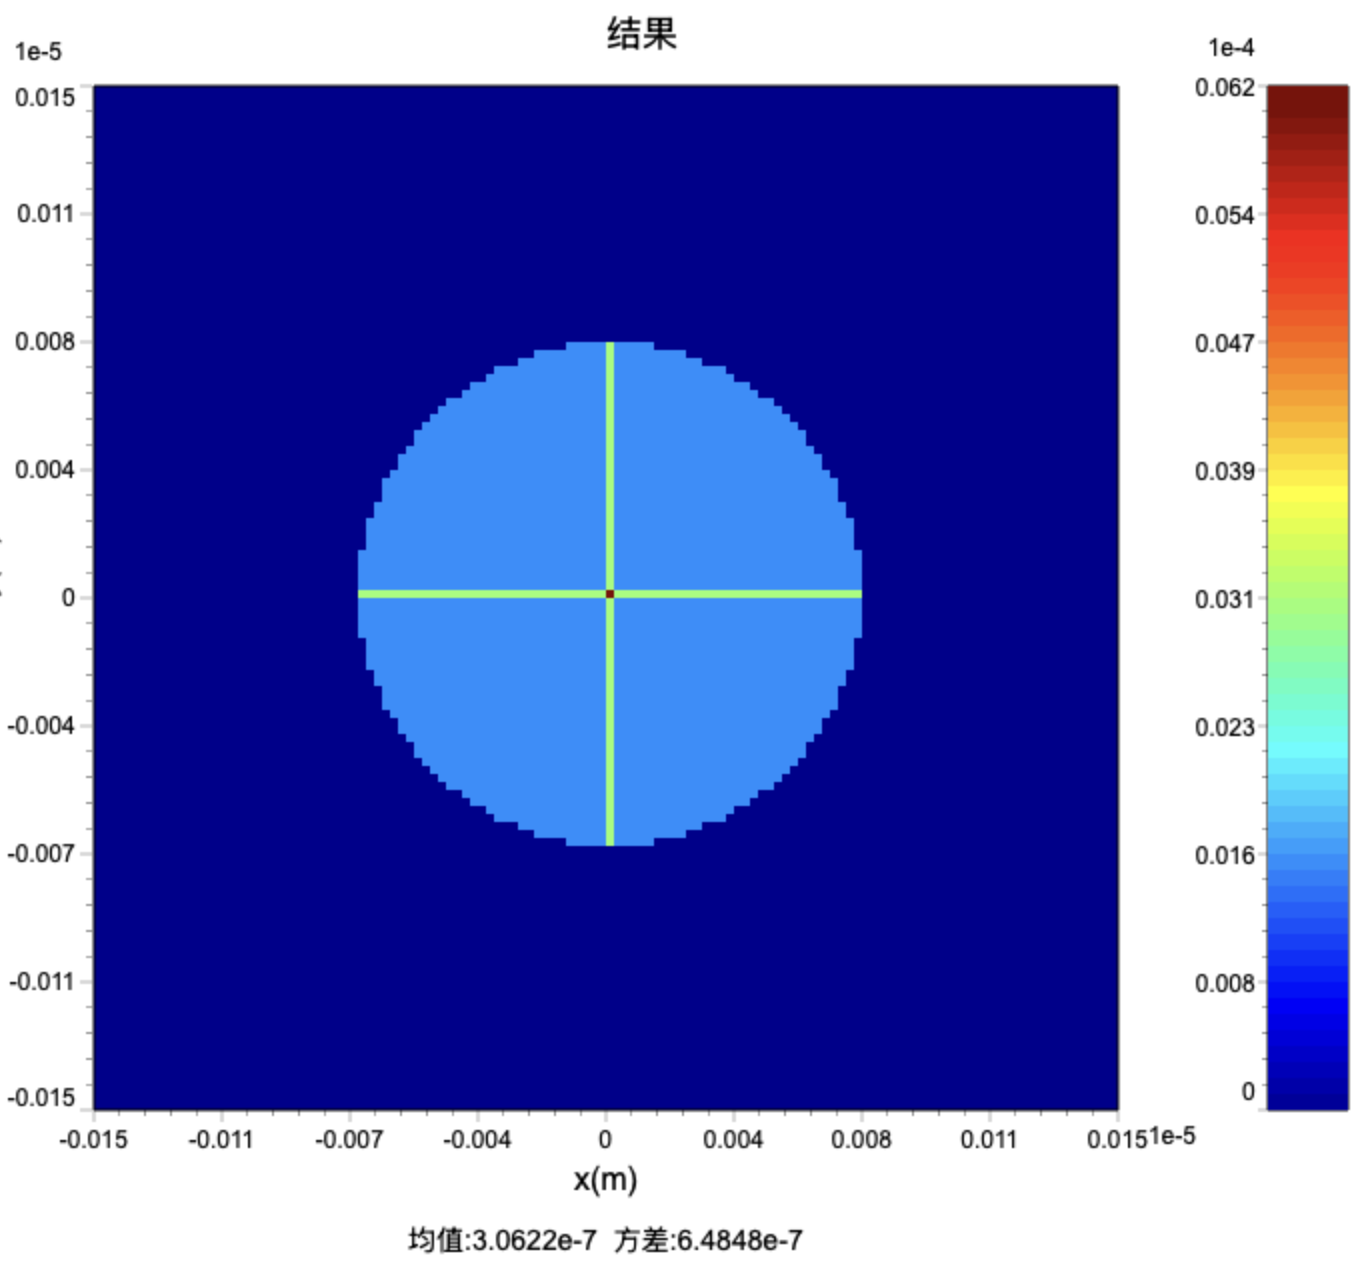
\includegraphics[width=0.3\textwidth]{Figure_3.3.png} 
    \caption{$632.8~nm$图像}
    \label{Figure_3.3} 
 \end{figure}\\
 得到的$L_2$即为对应焦距
 
 \subsection{由横向放大率求顶物距和顶像距}
 代入公式，求得放大/缩小对应的$L_1$，$L_2$如下：\\
 \begin{table}[h]
  \centering
   \begin{tabular}{|c|c|c|c|c|}
    \hline
    $m$ & $L_1$ & $L_2$ \\ 
    \hline
    $2$ & $73.773$ & $147.546$ \\
    \hline
    $\frac{1}{2}$ & $152.178$ & $76.089$ \\
    \hline
  \end{tabular}
  \caption{实验二参数}
  \label{Date_2}
 \end{table}\\
 \begin{figure}[h] 
    \centering
    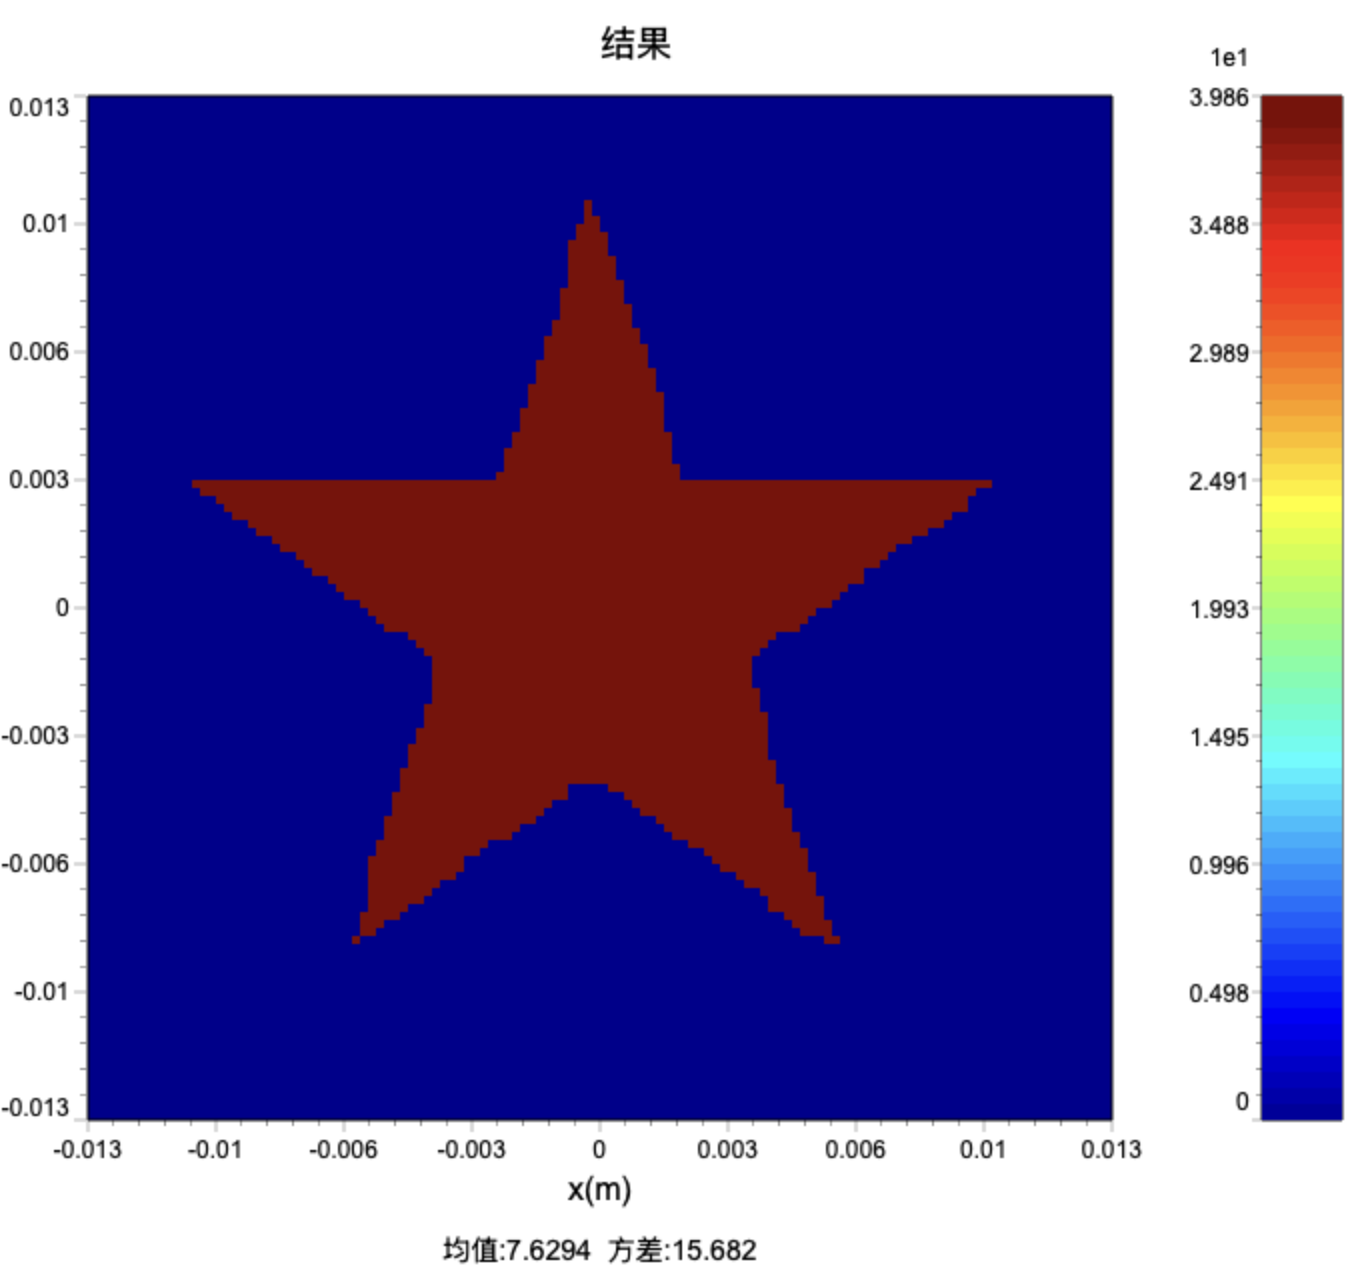
\includegraphics[width=0.4\textwidth]{Figure_3.4.png} 
    \caption{原图像}
    \label{Figure_3.4} 
 \end{figure}\\
 \begin{figure}[h] 
    \centering
    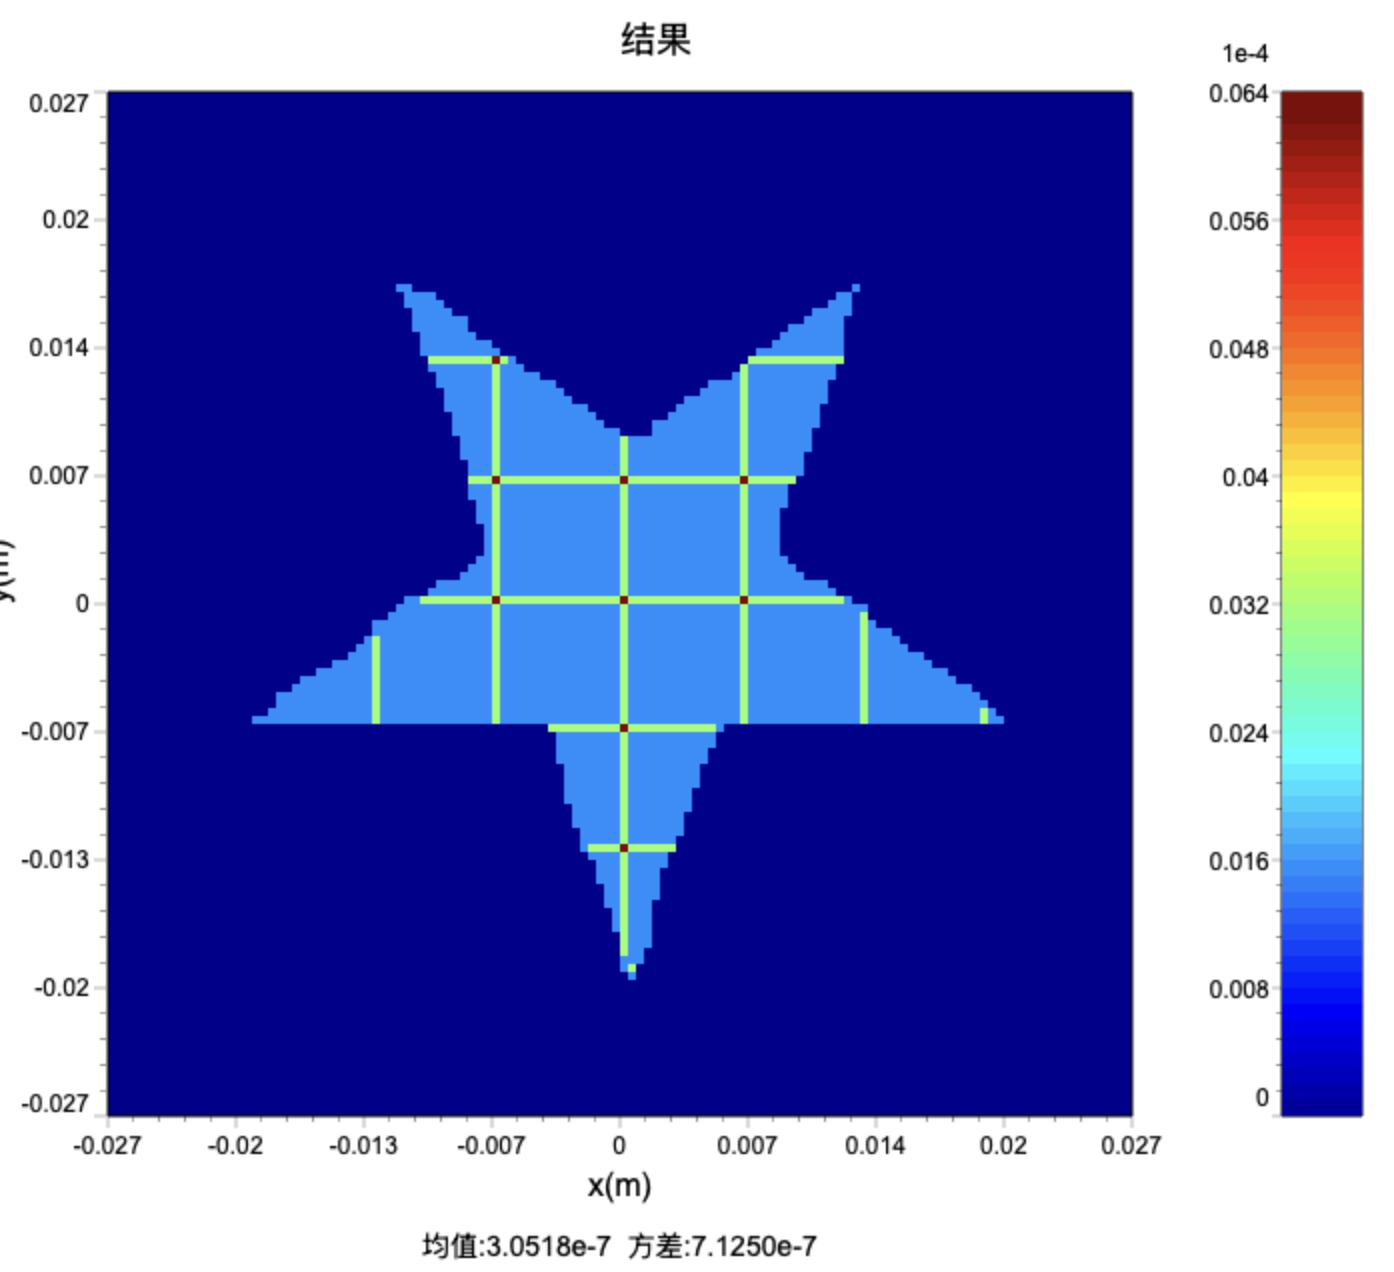
\includegraphics[width=0.4\textwidth]{Figure_3.5.png} 
    \caption{放大图像}
    \label{Figure_3.5} 
 \end{figure}\\
 \begin{figure}[h] 
    \centering
    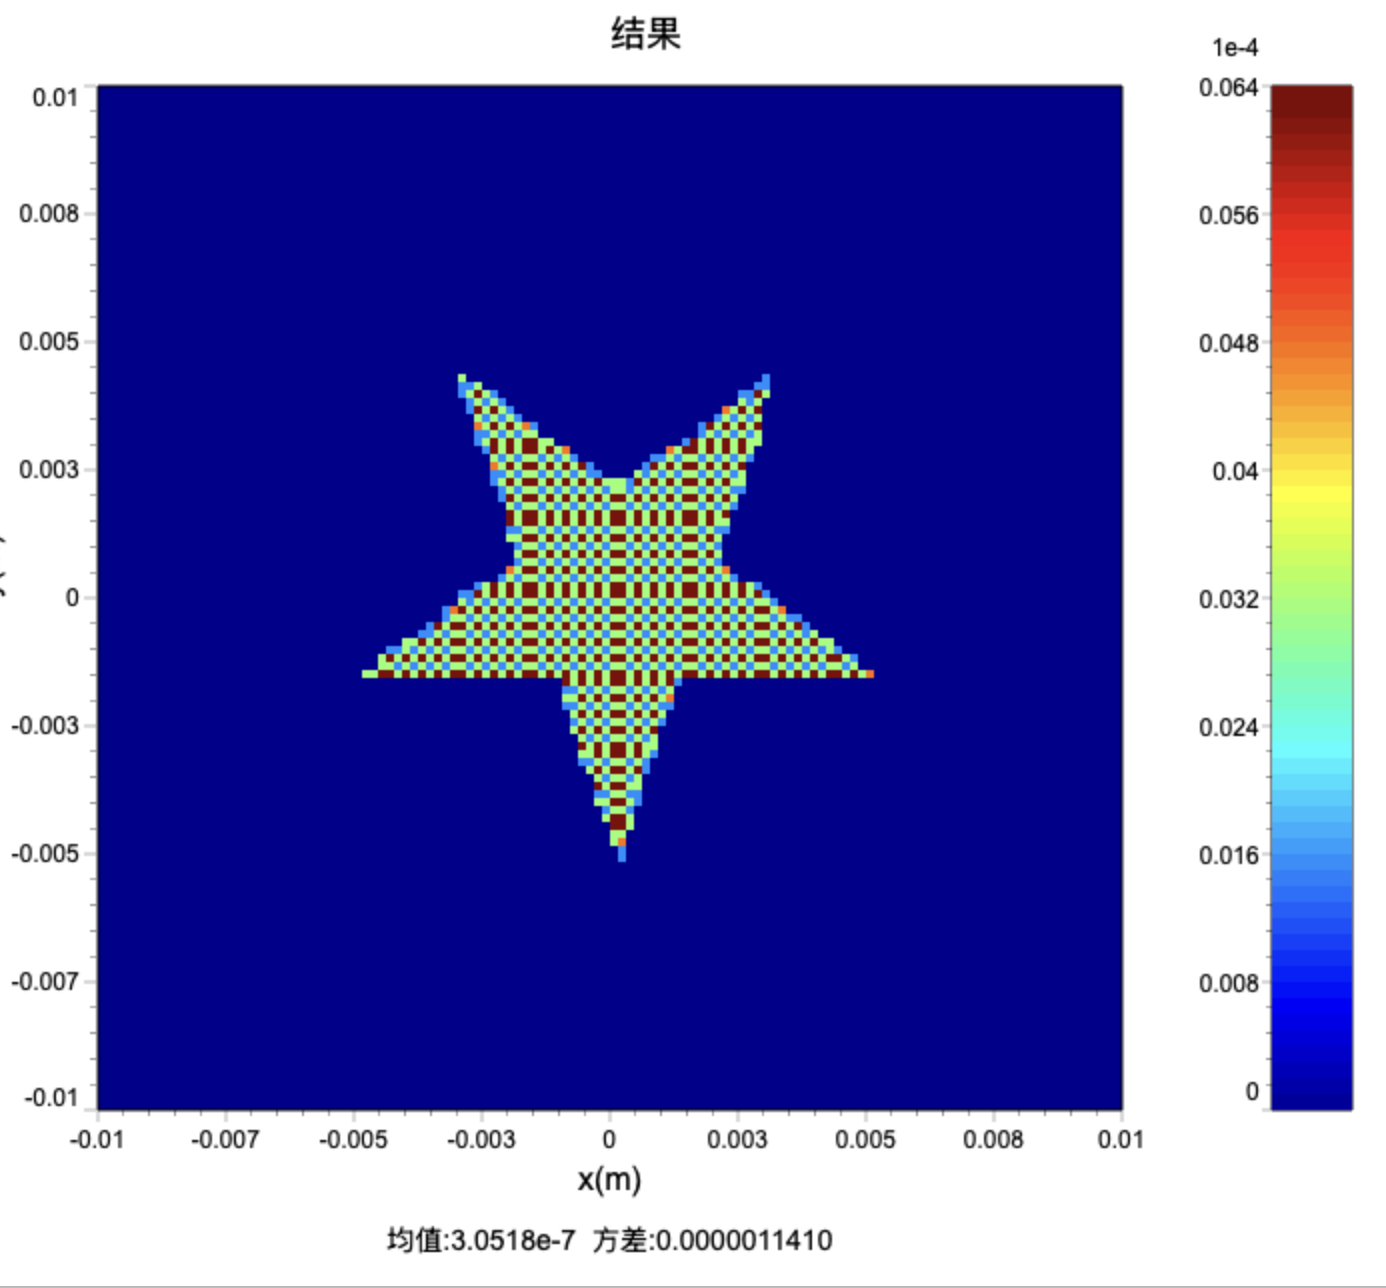
\includegraphics[width=0.4\textwidth]{Figure_3.6.png} 
    \caption{缩小图像}
    \label{Figure_3.6} 
 \end{figure}\\
 可以发现，放大/缩小图像的长度分别是原图的两倍，和二分之一，证明参数正确。
\end{document}